\documentclass[10pt,a4paper]{article}

\usepackage{graphicx}
\usepackage[left=2cm,right=2cm,top=2cm,bottom=2cm]{geometry}
\usepackage[usenames,dvipsnames,svgnames,table]{xcolor}
\usepackage{placeins}

\newenvironment{ttSection}{\ttfamily}{\par}


\begin{document}

%\section{Annotations}

%\begin{itemize}
%\item \texttt{@NonParadigm(type)} : 'data' or 'active'

%\end{itemize}
The key difference between Level~1 and Level~2 programs is the ability to nest mission sequencers inside missions, which creates a tiered program hierarchy. Each tier is formed of a series of clusters of missions and schedulables, where each mission in a tier is controlled by a mission sequencer in the tier above. The safelet and the top-level mission sequencers are contained in the control tier at the top of the hierarchy. As an example of the tiers within a program we consider the example in Figure~\ref{fig:AircraftDiagram}, which shows a program controlling an aircraft that has three modes of operation: take off, cruising, and landing.

\begin{figure}[!h]
\begin{center}
\includegraphics[scale=0.4]{AircraftStructure.png}
\caption{The processes in the model of the Aircraft mode change application \label{fig:AircraftDiagram}}
\end{center}
\end{figure}

The Control~Tier contains the $ACSafelet$ and $MainMissionSequencer$ classes. Tier~0 contains one cluster that pairs the $MainMission$ with the the four event handlers ($EnvMoniotr$, $FlightSensors$, $ControlHandler$, $CommsHandler$) and the $ACModeChanger$, which is the nested mission sequencer. This nested mission sequencer indicates that we need another tier, Tier~1.

Tier~1 contains three clusters. Each cluster pairs a single mission with the schedulable objects that it may register. One cluster pairs the $TakeOffMission$ with the $TakfeOffMonitor$, $LandingGearHandler$, and $TakeOffFailureHandler$. The second cluster pairs the $CruiseMission$ with the $NavigationHandler$ and $BeginLandingMonitor$. The final cluster pairs the $LandMission$ with the $SafeLandingHandler$, $LandingGearHandler$, $GroundDistanceMonitor$, and $InstrumentLandingSystemMonitor$. 

Because of this tiered structure in Level~2 programs, we approach the translation hierarchically. Figure~\ref{fig:translationFlow} shows a flowchart of the translation process. 

\begin{figure}[h!]
\begin{center}
\includegraphics[scale=0.5]{translation.pdf}
\caption{Flowchart of our Translation Process \label{fig:translationFlow} }
\end{center}
\end{figure}

At the top of the diagram we accept an SCJ program, compile it and analyse it, described briefly in Section~\ref{sec:analysis}. Then we begin the exploration phase, described in Section~\ref{sec:analysis}, in which we extract the information we require from the program. The hierarchy of an SCJ program can be seen as a tree, with the safelet as the root element. The analysis phase, gives us the elements in the tree, but not its structure, so we start with the safelet and use the objects in the program to build the tree's structure. Once we have explored the tree of objects in the program and extracted the information we need, we move on to the translation phase -- described in Section~\ref{sec:translation}.

\section{Analysis}
\label{sec:analysis}

In the current tool, the analysis phase takes an SCJ program, compiles it, and analyses it. The output of this phase is a list of trees the represent the classes. Since this is SCJ agnostic, we intend to reuse this functionality. To check that this functionality can be reused without causing problems, we have compiled and analysed a simple Level~2 program using the current implementation of the tool. The list of trees is used during the exploration phase, which we describe next.

\section{Exploration}
\label{sec:exploration}


The safelet can be identified easily because there is only one in the program. We retrieve the possible top-level mission sequencers and then begin a loop in the flow of exploring the program. For each top-level mission sequencer, we explore all of the missions that it can return. In doing so we explore each mission and its schedulables in turn, before moving on to the next mission sequencer. 

Because the analysis phase outputs a representation of each class in the program as tree, we use the visitor pattern to traverse the different types of element that we might find in each tree and extract the variables and the contents of the methods that we need for our translation, which we describe in Section~\ref{sec:translation}.

Upon discovery, each object (apart from the safelet) is assigned a unique identifier based upon the class's name -- multiple instances of a class result in multiple identifiers. This identifier is used in our model as a parameter to the processes representing that class. The location of the discovered objects within the program is important for the translation and is also recorded.

\subsection{Find and Visit Safelet}

Because there is only one safelet in a program, to find the program's safelet we search the list of class trees returned by the analysis phase and identify the class that implements \texttt{javax.safetycritical.Safelet}. Once the safelet is identified, we visit it and extract the contents of the \texttt{initializeApplication()} and \texttt{getSequencer()} methods, as well as any program-defined methods and variables. 

The \texttt{getSequencer()} method returns classes that extend \texttt{javax.safetycritical.MissionSequencer}. These classes are the top-level mission sequencers and their names are collected and used in the next stage of the translation. 

Finally, the name of the safelet class is recorded for use in the translation of the high-level network of the processes in the model. Next we visit the top-level mission sequencers.

\subsection{Visit Sequencer}
\label{sec:sequencer}
This stage makes use of the top-level sequencer names recorded as the return values from the safelet's \texttt{getSequencer()} method, it is also used to translate any nested mission sequencers that are found during the visiting of schedulables. We discus nested mission sequencers further in Section~\ref{sec:schedulables}. Because we build the tree of an SCJ program depth-first, if there are no more top-level mission sequencers to visit then we have explored the whole program and we can proceed to the translation phase, described in Section~\ref{sec:translation}.

When visiting a mission sequencer we capture the contents of the \texttt{getNextMission()} method and any program-specific methods and variables. Similarly to visiting the safelet, we collect the return values of the \texttt{getNextMission()} method for use in the next stage of the translation. 

Finally, we record the name of this sequencer and its location in the hierarchy. If it is returned by the safelet's \texttt{getSequencer()} method, then is is a top-level sequencer. If it is returned by a mission, then it is a nested mission sequencer. Either type of mission sequencer is recorded in it's relevant tier.

\subsection{Visit Mission}

This translation stage makes use of the collected names of the missions returned by the \texttt{getNextMission()} method of a mission sequencer. We visit each mission returned by a particular mission sequencer and each of that mission's schedulables before moving on to the next mission. This is because we pair each mission with its schedulables to form a cluster. 

When visiting a mission we capture the contents of the \texttt{initialize()} and \texttt{cleanUp()} methods, as well as any program-specific methods and variables. To find the schedulables of a mission we find any class that may be registered during the mission's \texttt{initialize()} method. The names of these classes are collected and used in the next stage of the translation. 

We record the name of this mission, in preparation for pairing it with its schedulables as a cluster. We also record where in the hierarchy this mission resides. For example, if it is returned by a top-level mission sequencer, then it resides in Tier 0. 

\subsection{Visit Schedulable}
\label{sec:schedulables}

This stage of the translation takes a collection of names of the schedulables registered in a mission's \texttt{initialize()} method. We visit each schedulable in turn and check if it is a nested mission sequencer or some other kind of schedulable by checking if the schedulable extends \texttt{javax.safetycritical.MissionSequencer}. If the schedulable is a mission sequencer, then we use the same method described in Section~\ref{sec:sequencer}. Otherwise, we check if the schedulable is a managed thread or one of the three kinds of event handler.

When visiting a schedulable, which isn't a mission sequencer, we capture the \texttt{handleAsyncEvent()} method for event handlers or the \texttt{run()} method for managed threads, as well as any program-specific methods and variables. 

When visiting a nested mission sequencer we visit the mission sequencer and then begin visiting its missions and their schedulables. A nested mission sequencer indicates a new tier in the program's hierarchy. 

When we are visiting a mission's event handler or managed thread, we continue visiting schedulables from that mission until there are none left (or we find a mission sequencer) and then we move on to the next mission returned by the mission sequencer directly about this schedulable.

%what?
Once the mission sequencer in question has no more missions to explore, we return to the next mission sequencer about our current position. Once there are no more top-level mission sequencers we have explored all of the paradigm objects in the program and we can move on to the translation proper, described in the Section~\ref{sec:translation}.

\subsection{Non-Paradigm Objects}

Non-paradigm objects are objects in the program that do not extend classes or implement interfaces from the SCJ API. During the hierarchical exploration of the program, if any non-paradigm objects are instantiated then they are visited with a special visitor and their name is recorded separately.


\subsection{Components making Non-paradigm Method Calls}

A non-paradigm method call is when a method is called that is not specified in the infrastructure of SCJ, but is program-specific. Because we need to model them differently, we must identify when components make non-paradigm method calls. They can only occur during program-specific code, so we check each method called in application code to see if the class it is declared in is in the SCJ API or not. For methods that are in the SCJ API, they are paradigm method calls. Methods that are declared in the program are non-paradigm method calls. 

For example:
\begin{ttSection}
For each methodCall in applicationMethod, \\
if methodCall's declared class is not javax.safetycritical.Mission \\
then record it as non-paradigm\\
else\\
continue
\end{ttSection}


\section{Translate}
\label{sec:translation}

Translation occures in two stages, low-level and high-level. The low-level translation translates the information gthered about each of the classes in the program during the previous stages and produces the processes that represent them in our model. The high-level translation translates the information gathered about the program hierarchy and translates it into the clusters and tiers that make up the network of the processes that organises our model at the top-level.

Both stages of the translation are achieved using the Freemarker template engine, which takes a data model and a template and combines them to produce output. For the low-level translation, the information gathered from visiting each class in the program (as we described above) is used to produce a data model for that class. The relevant template is loaded and combined with the data model to produce our model. For the high-level translation, the information record by each visitor about the position int he hierarchy of the class it is visiting is used to construct a data model, the template is selected and combined with the data model to produce the high-level network that controls the processes in our model.


\end{document}